\textbf{Benchmarking. } This project sets the theoretical framework, therefore the next step is to optimise the model for benchmarking to prove real world usefulness. Benchmarking results of CMACE should be impressive as it matches all the theoretical properties of MACE which provided state-of-the-art results. The main optimisation problems are as follows:

\begin{itemize}
    \item Add in layer normalisation to ensure that values to not grow arbitrarily large after many layers
    \item Add in regularisation techniques such as penalising the size of parameters to prevent overfitting
    \item Tune the hyperparameters such as the number of layers, number of channels, maximum tensor rank via grid search
    \item Find computational improvements. For example, by compiling the model using PyTorch \texttt{TorchScript} framework 
\end{itemize}

After these improvements are done, benchmarking against popular molecular benchmarks such as QM9 and MD17 can be used to gauge model performance. 

\textbf{Anti-symmetric Contractions. } Currently in CMACE, all contractions are symmetric. This is a desired property when measuring physical properties of a single molecule such as energy which should not change on inversion as CMACE produces scalars with even parity which don't change on inversion. Although in multi-molecule applications it is useful to have pseudoscalars which flip sign on inversion. This is becuase, molecules with chiral carbons have two versions which are non-superimposable mirror images. For example, one version of limonene smells like lemons whereas its mirror image smells of pine trees illustrating how they differently interact with smell receptors. Therefore in this multi-molecule case is desirable to have pseudoscalars that have odd parity under inversion such that the model can vary its outputs depending on which mirror images are used. 

\begin{figure}[H]
    \centering
    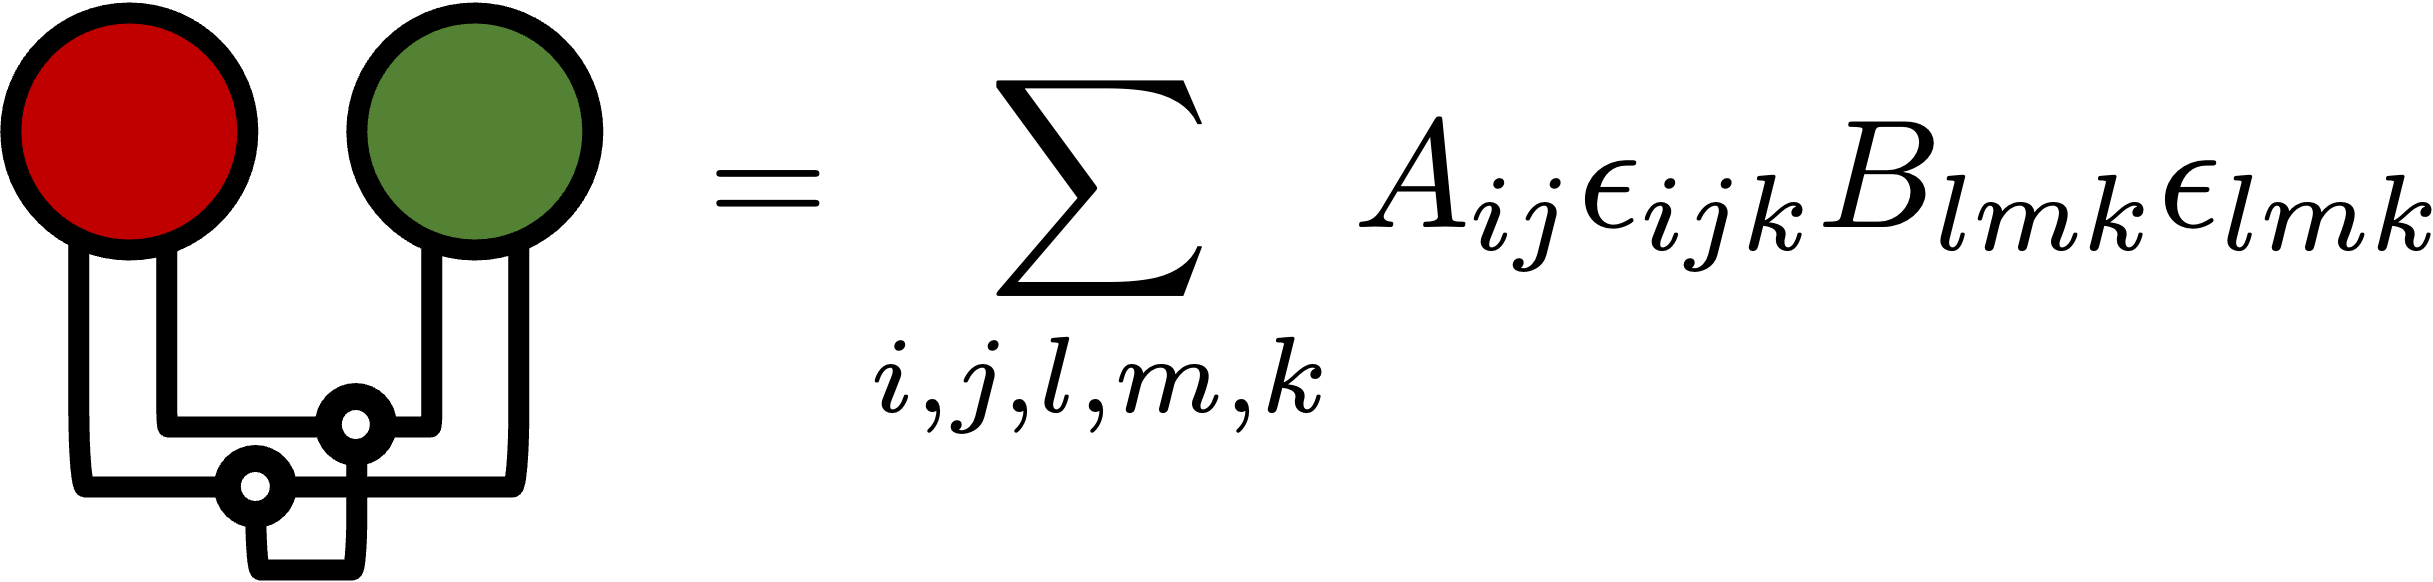
\includegraphics[width=0.5\textwidth]{figures/anti-sym.png}
    \caption{Anti-symmetric contraction using the Levi-Cevita tensor - denoted by small white circle. Allows for the production of odd parity pseudoscalars which are important for representing interactions between multiple molecules with chirality}
    \label{fig:anti-sym}
\end{figure}

This requires the use of a `dual' set of features that are contracted anti-symmetrically using the Levi-Civita tensor $\epsilon_{ijk}$. Figure \ref{fig:anti-sym} shows how these anti-symmetric contractions can be represented in tensor network notation. 




